%% slides_clinical.tex -- clinician-oriented version (~16 main slides + technical backup)
%% Put this file in the slides/ folder (next to figs/ and tables/), then:
%%   pdflatex slides_clinical.tex && pdflatex slides_clinical.tex
%\documentclass[aspectratio=169,11pt]{beamer}
%\usetheme{Madrid}
%\setbeamertemplate{navigation symbols}{}
%\usepackage[T1]{fontenc}
%\usepackage{lmodern}
%\usepackage{amsmath,amssymb,booktabs,graphicx}
%
%\makeatletter
%\newcommand{\res}[1]{\@ifundefined{res@#1}{\textbf{??}}{\@nameuse{res@#1}}}
%\makeatother
%\newcommand{\safeinput}[1]{\IfFileExists{#1}{\input{#1}}{\fbox{\footnotesize missing: \texttt{\detokenize{#1}}}}}
%\newcommand{\safegraphic}[2]{\IfFileExists{#2}{\includegraphics[#1]{#2}}{\fbox{\parbox{0.5\linewidth}{\centering\footnotesize missing: \texttt{\detokenize{#2}}}}}}
%\IfFileExists{tables/numbers.tex}{\makeatletter
\@namedef{res@A-aucb-ALL}{0.625}
\@namedef{res@A-aucb-gaussian}{0.669}
\@namedef{res@A-aucb-hotspot}{0.543}
\@namedef{res@A-aucb-linear}{0.980}
\@namedef{res@A-aucb-periodic}{0.527}
\@namedef{res@A-aucbeta}{0.625}
\@namedef{res@A-aucp-ALL}{0.505}
\@namedef{res@A-aucp-gaussian}{0.511}
\@namedef{res@A-aucp-hotspot}{0.477}
\@namedef{res@A-aucp-linear}{0.876}
\@namedef{res@A-aucp-periodic}{0.391}
\@namedef{res@A-aucpip}{0.505}
\@namedef{res@A-called}{673}
\@namedef{res@A-f1}{0.141}
\@namedef{res@A-fn}{77}
\@namedef{res@A-fp}{594}
\@namedef{res@A-ngenes}{1,500}
\@namedef{res@A-ntrue}{132}
\@namedef{res@A-nunits}{1,316}
\@namedef{res@A-prec}{0.085}
\@namedef{res@A-rate-adip}{42\%}
\@namedef{res@A-rate-ctsv}{73\%}
\@namedef{res@A-rate-marker}{47\%}
\@namedef{res@A-rate-null}{44\%}
\@namedef{res@A-rate-svgaussian}{33\%}
\@namedef{res@A-rate-svhotspot}{41\%}
\@namedef{res@A-rate-svlinear}{94\%}
\@namedef{res@A-rate-svperiodic}{30\%}
\@namedef{res@A-rec}{0.417}
\@namedef{res@A-runtime}{23.0}
\@namedef{res@A-topk}{0.250}
\@namedef{res@A-tp}{55}
\@namedef{res@B-aucb-ALL}{0.569}
\@namedef{res@B-aucb-gaussian}{0.629}
\@namedef{res@B-aucb-hotspot}{0.553}
\@namedef{res@B-aucb-linear}{0.930}
\@namedef{res@B-aucb-periodic}{0.410}
\@namedef{res@B-aucbeta}{0.569}
\@namedef{res@B-aucp-ALL}{0.507}
\@namedef{res@B-aucp-gaussian}{0.532}
\@namedef{res@B-aucp-hotspot}{0.492}
\@namedef{res@B-aucp-linear}{0.806}
\@namedef{res@B-aucp-periodic}{0.393}
\@namedef{res@B-aucpip}{0.507}
\@namedef{res@B-called}{859}
\@namedef{res@B-f1}{0.149}
\@namedef{res@B-fn}{60}
\@namedef{res@B-fp}{761}
\@namedef{res@B-ngenes}{1,500}
\@namedef{res@B-ntrue}{132}
\@namedef{res@B-nunits}{1,316}
\@namedef{res@B-prec}{0.086}
\@namedef{res@B-rate-adip}{56\%}
\@namedef{res@B-rate-ctsv}{79\%}
\@namedef{res@B-rate-marker}{58\%}
\@namedef{res@B-rate-null}{57\%}
\@namedef{res@B-rate-svgaussian}{58\%}
\@namedef{res@B-rate-svhotspot}{53\%}
\@namedef{res@B-rate-svlinear}{94\%}
\@namedef{res@B-rate-svperiodic}{39\%}
\@namedef{res@B-rec}{0.545}
\@namedef{res@B-runtime}{2.1}
\@namedef{res@B-topk}{0.167}
\@namedef{res@B-tp}{72}
\@namedef{res@C-aucb-ALL}{0.760}
\@namedef{res@C-aucb-gaussian}{0.874}
\@namedef{res@C-aucb-hotspot}{0.659}
\@namedef{res@C-aucb-linear}{0.998}
\@namedef{res@C-aucb-periodic}{0.662}
\@namedef{res@C-aucbeta}{0.760}
\@namedef{res@C-aucp-ALL}{0.734}
\@namedef{res@C-aucp-gaussian}{0.773}
\@namedef{res@C-aucp-hotspot}{0.643}
\@namedef{res@C-aucp-linear}{0.900}
\@namedef{res@C-aucp-periodic}{0.712}
\@namedef{res@C-aucpip}{0.734}
\@namedef{res@C-called}{785}
\@namedef{res@C-f1}{0.246}
\@namedef{res@C-fn}{22}
\@namedef{res@C-fp}{651}
\@namedef{res@C-ngenes}{1,500}
\@namedef{res@C-ntrue}{132}
\@namedef{res@C-nunits}{1,316}
\@namedef{res@C-prec}{0.145}
\@namedef{res@C-rate-adip}{55\%}
\@namedef{res@C-rate-ctsv}{73\%}
\@namedef{res@C-rate-marker}{48\%}
\@namedef{res@C-rate-null}{44\%}
\@namedef{res@C-rate-svgaussian}{89\%}
\@namedef{res@C-rate-svhotspot}{65\%}
\@namedef{res@C-rate-svlinear}{100\%}
\@namedef{res@C-rate-svperiodic}{87\%}
\@namedef{res@C-rec}{0.833}
\@namedef{res@C-runtime}{1.9}
\@namedef{res@C-topk}{0.364}
\@namedef{res@C-tp}{110}
\@namedef{res@D-aucb-ALL}{0.837}
\@namedef{res@D-aucb-gaussian}{0.915}
\@namedef{res@D-aucb-hotspot}{0.681}
\@namedef{res@D-aucb-linear}{0.997}
\@namedef{res@D-aucb-periodic}{0.836}
\@namedef{res@D-aucbeta}{0.837}
\@namedef{res@D-aucp-ALL}{0.705}
\@namedef{res@D-aucp-gaussian}{0.699}
\@namedef{res@D-aucp-hotspot}{0.562}
\@namedef{res@D-aucp-linear}{0.865}
\@namedef{res@D-aucp-periodic}{0.761}
\@namedef{res@D-aucpip}{0.705}
\@namedef{res@D-called}{525}
\@namedef{res@D-f1}{0.257}
\@namedef{res@D-fn}{49}
\@namedef{res@D-fp}{431}
\@namedef{res@D-ngenes}{1,500}
\@namedef{res@D-ntrue}{132}
\@namedef{res@D-nunits}{1,316}
\@namedef{res@D-prec}{0.161}
\@namedef{res@D-rate-adip}{36\%}
\@namedef{res@D-rate-ctsv}{33\%}
\@namedef{res@D-rate-marker}{30\%}
\@namedef{res@D-rate-null}{31\%}
\@namedef{res@D-rate-svgaussian}{61\%}
\@namedef{res@D-rate-svhotspot}{38\%}
\@namedef{res@D-rate-svlinear}{88\%}
\@namedef{res@D-rate-svperiodic}{74\%}
\@namedef{res@D-rec}{0.629}
\@namedef{res@D-runtime}{9.4}
\@namedef{res@D-topk}{0.439}
\@namedef{res@D-tp}{83}
\@namedef{res@E-aucb-ALL}{0.809}
\@namedef{res@E-aucb-gaussian}{0.915}
\@namedef{res@E-aucb-hotspot}{0.670}
\@namedef{res@E-aucb-linear}{0.997}
\@namedef{res@E-aucb-periodic}{0.765}
\@namedef{res@E-aucbeta}{0.809}
\@namedef{res@E-aucp-ALL}{0.732}
\@namedef{res@E-aucp-gaussian}{0.804}
\@namedef{res@E-aucp-hotspot}{0.627}
\@namedef{res@E-aucp-linear}{0.786}
\@namedef{res@E-aucp-periodic}{0.735}
\@namedef{res@E-aucpip}{0.732}
\@namedef{res@E-called}{300}
\@namedef{res@E-f1}{0.317}
\@namedef{res@E-fn}{65}
\@namedef{res@E-fp}{224}
\@namedef{res@E-ngenes}{1,500}
\@namedef{res@E-ntrue}{132}
\@namedef{res@E-nunits}{1,316}
\@namedef{res@E-prec}{0.230}
\@namedef{res@E-rate-adip}{18\%}
\@namedef{res@E-rate-ctsv}{27\%}
\@namedef{res@E-rate-marker}{16\%}
\@namedef{res@E-rate-null}{16\%}
\@namedef{res@E-rate-svgaussian}{58\%}
\@namedef{res@E-rate-svhotspot}{32\%}
\@namedef{res@E-rate-svlinear}{69\%}
\@namedef{res@E-rate-svperiodic}{52\%}
\@namedef{res@E-rec}{0.508}
\@namedef{res@E-runtime}{9.7}
\@namedef{res@E-topk}{0.424}
\@namedef{res@E-tp}{67}
\@namedef{res@F-aucbeta}{0.999}
\@namedef{res@F-aucpip}{0.996}
\@namedef{res@F-called}{590}
\@namedef{res@F-f1}{0.917}
\@namedef{res@F-fn}{0}
\@namedef{res@F-fp}{90}
\@namedef{res@F-fphub}{0.191}
\@namedef{res@F-lam}{0.0826}
\@namedef{res@F-lam23}{0.190}
\@namedef{res@F-ngenes}{5,000}
\@namedef{res@F-nnonhub}{4,410}
\@namedef{res@F-nnullhub}{90}
\@namedef{res@F-nonhub}{17}
\@namedef{res@F-ntrue}{500}
\@namedef{res@F-nullhub}{73}
\@namedef{res@F-nunits}{1,024}
\@namedef{res@F-prec}{0.847}
\@namedef{res@F-rec}{1.000}
\@namedef{res@F-runtime}{16.3}
\@namedef{res@F-topk}{0.978}
\@namedef{res@F-tp}{500}
\@namedef{res@G-aucbeta}{1.000}
\@namedef{res@G-aucpip}{0.976}
\@namedef{res@G-called}{953}
\@namedef{res@G-f1}{0.688}
\@namedef{res@G-fn}{0}
\@namedef{res@G-fp}{453}
\@namedef{res@G-fphub}{0.055}
\@namedef{res@G-lam}{0.0367}
\@namedef{res@G-lam23}{0.111}
\@namedef{res@G-ngenes}{5,000}
\@namedef{res@G-nnonhub}{4,410}
\@namedef{res@G-nnullhub}{90}
\@namedef{res@G-nonhub}{434}
\@namedef{res@G-ntrue}{500}
\@namedef{res@G-nullhub}{19}
\@namedef{res@G-nunits}{1,024}
\@namedef{res@G-prec}{0.525}
\@namedef{res@G-rec}{1.000}
\@namedef{res@G-runtime}{16.1}
\@namedef{res@G-topk}{0.998}
\@namedef{res@G-tp}{500}
\@namedef{res@fig-nbins}{101,000}
\@namedef{res@fig-ngenes}{18,000}
\@namedef{res@fit-nbins}{20,000}
\@namedef{res@fit-ngenes}{4,000}
\@namedef{res@ours-cpg}{0.37}
\@namedef{res@paper-cpg}{20.5}
\@namedef{res@paper-f1}{0.996}
\@namedef{res@paper-nbins}{1,024}
\@namedef{res@paper-ngenes}{5,000}
\@namedef{res@paper-nsv}{500}
\@namedef{res@paper-prec}{1.000}
\@namedef{res@paper-rec}{0.992}
\@namedef{res@paper-scen}{linear pattern, star network, dropout 0.1}
\makeatother
}{}
%
%
%
%
%
%
%
%
%
%
%
%
%
%
%
%
%
%
%
%
%
%
%
%
%
%










\documentclass[10pt,aspectratio=169]{beamer}

% -------------------------------------------------------------------------
% NIH RDI-SIG Workshop talk, revised from JSM LaBay talk
% Prepared for Ali Reza Taheriyoun, PhD
% -------------------------------------------------------------------------

\usetheme{CambridgeUS}
\usecolortheme{dolphin}
\usefonttheme{professionalfonts}
\usepackage[utf8]{inputenc}
\usepackage[T1]{fontenc}
\usepackage{lmodern}
\usepackage{microtype}
\usepackage{amsmath,amssymb,mathtools,bm}
\usepackage{booktabs,array,multirow}
\usepackage{graphicx}
\usepackage{xcolor}
\usepackage{hyperref}
\usepackage{listings}
\usepackage{ifthen}
\usepackage{animate}
\usepackage{layouts} 
\usepackage{gensymb}
\usepackage{lmodern}
\usepackage{fontawesome5}
%\usepackage{minted}

% Colors: GW-inspired palette, with NIH-compatible restraint
\definecolor{GWBlue}{RGB}{0,59,92}
\definecolor{GWGold}{RGB}{168,153,104}
\definecolor{DeepRed}{RGB}{170,35,35}
\definecolor{SoftGray}{RGB}{245,246,248}
\definecolor{DarkGray}{RGB}{72,72,72}
\definecolor{Forest}{RGB}{0,105,92}
\definecolor{mgtxnavy}{HTML}{193B52}
\definecolor{mgtxteal}{HTML}{168D91}
\definecolor{mgtxred}{HTML}{C95D5D}
\definecolor{mgtxamber}{HTML}{DDA84B}

\hypersetup{pdfpagemode=FullScreen,colorlinks=true,linkcolor=GWBlue,urlcolor=GWBlue}
\setbeamertemplate{navigation symbols}{}
\setbeamertemplate{caption}[numbered]


\lstdefinestyle{Rstyle}{
	language=R,
	% Background & frame
	backgroundcolor=\color{GWBlue!92!black},
	frame=none,
	% Fonts
	basicstyle=\ttfamily\footnotesize\color{white},
	% Syntax colors
	keywordstyle=\color{GWGold}\bfseries,
	stringstyle=\color{green!60!white},
	commentstyle=\color{gray!60}\itshape,
	identifierstyle=\color{white},
	% Line numbers
	numbers=left,
	numberstyle=\tiny\color{GWGold!60},
	numbersep=8pt,
	stepnumber=1,
	% Layout
	showstringspaces=false,
	breaklines=true,
	breakatwhitespace=true,
	tabsize=2,
	xleftmargin=14pt,
	xrightmargin=4pt,
	aboveskip=6pt,
	belowskip=2pt,
	% R keywords
	morekeywords={TRUE,FALSE,NULL,NA,Inf,NaN,
		library,require,source,
		function,if,else,for,while,repeat,
		return,next,break},
	% Operator highlighting
	literate=
	{<-}{{\color{GWGold!80}<-}}2
	{->}{{\color{GWGold!80}->}}2
	{==}{{\color{GWGold!80}==}}2
	{!=}{{\color{GWGold!80}!=}}2
	{>=}{{\color{GWGold!80}>=}}2
	{<=}{{\color{GWGold!80}<=}}2
	{\%in\%}{{\color{GWGold!80}\%in\%}}5
	{\%>\%}{{\color{GWGold!80}\%>\%}}3,
}
\setbeamercolor*{palette primary}{bg=GWBlue, fg=white}
\setbeamercolor*{palette secondary}{bg=GWGold, fg=black}
\setbeamercolor*{palette tertiary}{bg=GWBlue, fg=white}
\setbeamercolor*{titlelike}{fg=GWBlue}
\setbeamercolor*{title}{bg=GWBlue, fg=white}
\setbeamercolor*{frametitle}{fg=GWBlue,bg=white}
\setbeamercolor*{item}{fg=DeepRed}
\setbeamercolor*{block title}{bg=GWBlue,fg=white}
\setbeamercolor*{block body}{bg=SoftGray,fg=black}
\setbeamercolor*{alerted text}{fg=DeepRed}

\setbeamerfont{title}{size=\Large,series=\bfseries}
\setbeamerfont{subtitle}{size=\normalsize}
\setbeamerfont{author}{size=\normalsize}
\setbeamerfont{institute}{size=\small}
\setbeamerfont{date}{size=\small}
\setbeamerfont{frametitle}{size=\large,series=\bfseries}
\setbeamerfont{footnote}{size=\tiny}

\newcommand{\LaBay}{\texttt{LaBay}}
\newcommand{\cpGLMM}{\texttt{cpGLMM}}
\newcommand{\MGTX}{\textsc{MGTX}}
\newcommand{\Pred}{\mathrm{Pred}}
\newcommand{\ETTX}{\mathrm{ETTX}}
\newcommand{\source}[1]{\vspace{1mm}\par{\tiny\color{DarkGray}Source: #1}}
\newcommand{\speaker}[1]{\par{\tiny\color{DarkGray}\textbf{Speaker note.} #1}}
\newcommand{\takehome}[1]{\begin{block}{Take-home}\small #1\end{block}}

% Placeholder-safe figure macro: compile even when the original figures folder is absent.
\newcommand{\maybefig}[3]{%
	\IfFileExists{#1}{\includegraphics[#2]{#1}}{%
		\fbox{\begin{minipage}[c][#3][c]{0.94\linewidth}\centering\small\color{DarkGray}
				Placeholder for figure: \texttt{#1}\\[-1mm]
				\scriptsize Insert the corresponding manuscript/JSM figure here if available.
		\end{minipage}}%
	}%
}

\usepackage{amsmath,amssymb,booktabs,graphicx}

\makeatletter
\newcommand{\res}[1]{\@ifundefined{res@#1}{\textbf{??}}{\@nameuse{res@#1}}}
\makeatother
\newcommand{\safeinput}[1]{\IfFileExists{#1}{\input{#1}}{\fbox{\footnotesize missing: \texttt{\detokenize{#1}}}}}
\newcommand{\safegraphic}[2]{\IfFileExists{#2}{\includegraphics[#1]{#2}}{\fbox{\parbox{0.5\linewidth}{\centering\footnotesize missing: \texttt{\detokenize{#2}}}}}}
\IfFileExists{tables/numbers.tex}{\makeatletter
\@namedef{res@A-aucb-ALL}{0.625}
\@namedef{res@A-aucb-gaussian}{0.669}
\@namedef{res@A-aucb-hotspot}{0.543}
\@namedef{res@A-aucb-linear}{0.980}
\@namedef{res@A-aucb-periodic}{0.527}
\@namedef{res@A-aucbeta}{0.625}
\@namedef{res@A-aucp-ALL}{0.505}
\@namedef{res@A-aucp-gaussian}{0.511}
\@namedef{res@A-aucp-hotspot}{0.477}
\@namedef{res@A-aucp-linear}{0.876}
\@namedef{res@A-aucp-periodic}{0.391}
\@namedef{res@A-aucpip}{0.505}
\@namedef{res@A-called}{673}
\@namedef{res@A-f1}{0.141}
\@namedef{res@A-fn}{77}
\@namedef{res@A-fp}{594}
\@namedef{res@A-ngenes}{1,500}
\@namedef{res@A-ntrue}{132}
\@namedef{res@A-nunits}{1,316}
\@namedef{res@A-prec}{0.085}
\@namedef{res@A-rate-adip}{42\%}
\@namedef{res@A-rate-ctsv}{73\%}
\@namedef{res@A-rate-marker}{47\%}
\@namedef{res@A-rate-null}{44\%}
\@namedef{res@A-rate-svgaussian}{33\%}
\@namedef{res@A-rate-svhotspot}{41\%}
\@namedef{res@A-rate-svlinear}{94\%}
\@namedef{res@A-rate-svperiodic}{30\%}
\@namedef{res@A-rec}{0.417}
\@namedef{res@A-runtime}{23.0}
\@namedef{res@A-topk}{0.250}
\@namedef{res@A-tp}{55}
\@namedef{res@B-aucb-ALL}{0.569}
\@namedef{res@B-aucb-gaussian}{0.629}
\@namedef{res@B-aucb-hotspot}{0.553}
\@namedef{res@B-aucb-linear}{0.930}
\@namedef{res@B-aucb-periodic}{0.410}
\@namedef{res@B-aucbeta}{0.569}
\@namedef{res@B-aucp-ALL}{0.507}
\@namedef{res@B-aucp-gaussian}{0.532}
\@namedef{res@B-aucp-hotspot}{0.492}
\@namedef{res@B-aucp-linear}{0.806}
\@namedef{res@B-aucp-periodic}{0.393}
\@namedef{res@B-aucpip}{0.507}
\@namedef{res@B-called}{859}
\@namedef{res@B-f1}{0.149}
\@namedef{res@B-fn}{60}
\@namedef{res@B-fp}{761}
\@namedef{res@B-ngenes}{1,500}
\@namedef{res@B-ntrue}{132}
\@namedef{res@B-nunits}{1,316}
\@namedef{res@B-prec}{0.086}
\@namedef{res@B-rate-adip}{56\%}
\@namedef{res@B-rate-ctsv}{79\%}
\@namedef{res@B-rate-marker}{58\%}
\@namedef{res@B-rate-null}{57\%}
\@namedef{res@B-rate-svgaussian}{58\%}
\@namedef{res@B-rate-svhotspot}{53\%}
\@namedef{res@B-rate-svlinear}{94\%}
\@namedef{res@B-rate-svperiodic}{39\%}
\@namedef{res@B-rec}{0.545}
\@namedef{res@B-runtime}{2.1}
\@namedef{res@B-topk}{0.167}
\@namedef{res@B-tp}{72}
\@namedef{res@C-aucb-ALL}{0.760}
\@namedef{res@C-aucb-gaussian}{0.874}
\@namedef{res@C-aucb-hotspot}{0.659}
\@namedef{res@C-aucb-linear}{0.998}
\@namedef{res@C-aucb-periodic}{0.662}
\@namedef{res@C-aucbeta}{0.760}
\@namedef{res@C-aucp-ALL}{0.734}
\@namedef{res@C-aucp-gaussian}{0.773}
\@namedef{res@C-aucp-hotspot}{0.643}
\@namedef{res@C-aucp-linear}{0.900}
\@namedef{res@C-aucp-periodic}{0.712}
\@namedef{res@C-aucpip}{0.734}
\@namedef{res@C-called}{785}
\@namedef{res@C-f1}{0.246}
\@namedef{res@C-fn}{22}
\@namedef{res@C-fp}{651}
\@namedef{res@C-ngenes}{1,500}
\@namedef{res@C-ntrue}{132}
\@namedef{res@C-nunits}{1,316}
\@namedef{res@C-prec}{0.145}
\@namedef{res@C-rate-adip}{55\%}
\@namedef{res@C-rate-ctsv}{73\%}
\@namedef{res@C-rate-marker}{48\%}
\@namedef{res@C-rate-null}{44\%}
\@namedef{res@C-rate-svgaussian}{89\%}
\@namedef{res@C-rate-svhotspot}{65\%}
\@namedef{res@C-rate-svlinear}{100\%}
\@namedef{res@C-rate-svperiodic}{87\%}
\@namedef{res@C-rec}{0.833}
\@namedef{res@C-runtime}{1.9}
\@namedef{res@C-topk}{0.364}
\@namedef{res@C-tp}{110}
\@namedef{res@D-aucb-ALL}{0.837}
\@namedef{res@D-aucb-gaussian}{0.915}
\@namedef{res@D-aucb-hotspot}{0.681}
\@namedef{res@D-aucb-linear}{0.997}
\@namedef{res@D-aucb-periodic}{0.836}
\@namedef{res@D-aucbeta}{0.837}
\@namedef{res@D-aucp-ALL}{0.705}
\@namedef{res@D-aucp-gaussian}{0.699}
\@namedef{res@D-aucp-hotspot}{0.562}
\@namedef{res@D-aucp-linear}{0.865}
\@namedef{res@D-aucp-periodic}{0.761}
\@namedef{res@D-aucpip}{0.705}
\@namedef{res@D-called}{525}
\@namedef{res@D-f1}{0.257}
\@namedef{res@D-fn}{49}
\@namedef{res@D-fp}{431}
\@namedef{res@D-ngenes}{1,500}
\@namedef{res@D-ntrue}{132}
\@namedef{res@D-nunits}{1,316}
\@namedef{res@D-prec}{0.161}
\@namedef{res@D-rate-adip}{36\%}
\@namedef{res@D-rate-ctsv}{33\%}
\@namedef{res@D-rate-marker}{30\%}
\@namedef{res@D-rate-null}{31\%}
\@namedef{res@D-rate-svgaussian}{61\%}
\@namedef{res@D-rate-svhotspot}{38\%}
\@namedef{res@D-rate-svlinear}{88\%}
\@namedef{res@D-rate-svperiodic}{74\%}
\@namedef{res@D-rec}{0.629}
\@namedef{res@D-runtime}{9.4}
\@namedef{res@D-topk}{0.439}
\@namedef{res@D-tp}{83}
\@namedef{res@E-aucb-ALL}{0.809}
\@namedef{res@E-aucb-gaussian}{0.915}
\@namedef{res@E-aucb-hotspot}{0.670}
\@namedef{res@E-aucb-linear}{0.997}
\@namedef{res@E-aucb-periodic}{0.765}
\@namedef{res@E-aucbeta}{0.809}
\@namedef{res@E-aucp-ALL}{0.732}
\@namedef{res@E-aucp-gaussian}{0.804}
\@namedef{res@E-aucp-hotspot}{0.627}
\@namedef{res@E-aucp-linear}{0.786}
\@namedef{res@E-aucp-periodic}{0.735}
\@namedef{res@E-aucpip}{0.732}
\@namedef{res@E-called}{300}
\@namedef{res@E-f1}{0.317}
\@namedef{res@E-fn}{65}
\@namedef{res@E-fp}{224}
\@namedef{res@E-ngenes}{1,500}
\@namedef{res@E-ntrue}{132}
\@namedef{res@E-nunits}{1,316}
\@namedef{res@E-prec}{0.230}
\@namedef{res@E-rate-adip}{18\%}
\@namedef{res@E-rate-ctsv}{27\%}
\@namedef{res@E-rate-marker}{16\%}
\@namedef{res@E-rate-null}{16\%}
\@namedef{res@E-rate-svgaussian}{58\%}
\@namedef{res@E-rate-svhotspot}{32\%}
\@namedef{res@E-rate-svlinear}{69\%}
\@namedef{res@E-rate-svperiodic}{52\%}
\@namedef{res@E-rec}{0.508}
\@namedef{res@E-runtime}{9.7}
\@namedef{res@E-topk}{0.424}
\@namedef{res@E-tp}{67}
\@namedef{res@F-aucbeta}{0.999}
\@namedef{res@F-aucpip}{0.996}
\@namedef{res@F-called}{590}
\@namedef{res@F-f1}{0.917}
\@namedef{res@F-fn}{0}
\@namedef{res@F-fp}{90}
\@namedef{res@F-fphub}{0.191}
\@namedef{res@F-lam}{0.0826}
\@namedef{res@F-lam23}{0.190}
\@namedef{res@F-ngenes}{5,000}
\@namedef{res@F-nnonhub}{4,410}
\@namedef{res@F-nnullhub}{90}
\@namedef{res@F-nonhub}{17}
\@namedef{res@F-ntrue}{500}
\@namedef{res@F-nullhub}{73}
\@namedef{res@F-nunits}{1,024}
\@namedef{res@F-prec}{0.847}
\@namedef{res@F-rec}{1.000}
\@namedef{res@F-runtime}{16.3}
\@namedef{res@F-topk}{0.978}
\@namedef{res@F-tp}{500}
\@namedef{res@G-aucbeta}{1.000}
\@namedef{res@G-aucpip}{0.976}
\@namedef{res@G-called}{953}
\@namedef{res@G-f1}{0.688}
\@namedef{res@G-fn}{0}
\@namedef{res@G-fp}{453}
\@namedef{res@G-fphub}{0.055}
\@namedef{res@G-lam}{0.0367}
\@namedef{res@G-lam23}{0.111}
\@namedef{res@G-ngenes}{5,000}
\@namedef{res@G-nnonhub}{4,410}
\@namedef{res@G-nnullhub}{90}
\@namedef{res@G-nonhub}{434}
\@namedef{res@G-ntrue}{500}
\@namedef{res@G-nullhub}{19}
\@namedef{res@G-nunits}{1,024}
\@namedef{res@G-prec}{0.525}
\@namedef{res@G-rec}{1.000}
\@namedef{res@G-runtime}{16.1}
\@namedef{res@G-topk}{0.998}
\@namedef{res@G-tp}{500}
\@namedef{res@fig-nbins}{101,000}
\@namedef{res@fig-ngenes}{18,000}
\@namedef{res@fit-nbins}{20,000}
\@namedef{res@fit-ngenes}{4,000}
\@namedef{res@ours-cpg}{0.37}
\@namedef{res@paper-cpg}{20.5}
\@namedef{res@paper-f1}{0.996}
\@namedef{res@paper-nbins}{1,024}
\@namedef{res@paper-ngenes}{5,000}
\@namedef{res@paper-nsv}{500}
\@namedef{res@paper-prec}{1.000}
\@namedef{res@paper-rec}{0.992}
\@namedef{res@paper-scen}{linear pattern, star network, dropout 0.1}
\makeatother
}{}

\title[Spatially variable genes]{Finding genes with spatial patterns in tissue}
\subtitle{Testing a new statistical method on simulated tissue before using it on patient samples}
\author[AliReza Taheriyoun]{Ali R Taheriyoun, PhD}
\institute[GWU CBI]{Milken Institute School of Public Health, The George Washington University}
\date[\today]{Drs. Kaminski and Kusner Lab meeting}
%
%\title[Spatially variable genes]{Finding genes with spatial patterns in tissue}
%\subtitle{Testing a new statistical method on simulated tissue before using it on patient samples}
%\author{AliReza Taheriyoun}   % <-- edit
%\institute{Lab meeting}
%\date{\today}

\begin{document}

\begin{frame}
  \titlepage
\end{frame}
% ============================================================
% SLIDE 2 -- CORRECTED DATA AND INVENTORY
% ============================================================

\begin{frame}{Why this reprocessing was necessary}
	
	\begin{columns}[T]
		
		\column{0.5\textwidth}
		
		\small
		
		\textbf{Sample-identity investigation}
		
		\begin{itemize}
			\item External SNP-based QC raised concerns about
			sample labeling in the public RNA-seq dataset.
			
			\item A corrected-label delivery was prepared
			on November 17, 2026.
			
			\item The delivery documentation describes
			genotype comparisons using
			20,721 SNP loci.
			
			\item Original sequencing-core deliveries
			are preserved for traceability.
		\end{itemize}
		
		\vspace{-0.35cm}
		
		\begin{block}{Corrected sequencing inventory}
			\begin{itemize}
				\item 282 libraries; 93 participants
				\item 105 corrected labels
				\item 177 unchanged labels
				\item 31 previously missing M36 libraries recovered
			\end{itemize}
		\end{block}
		
		\column{0.55\textwidth}
		
		\begin{center}
			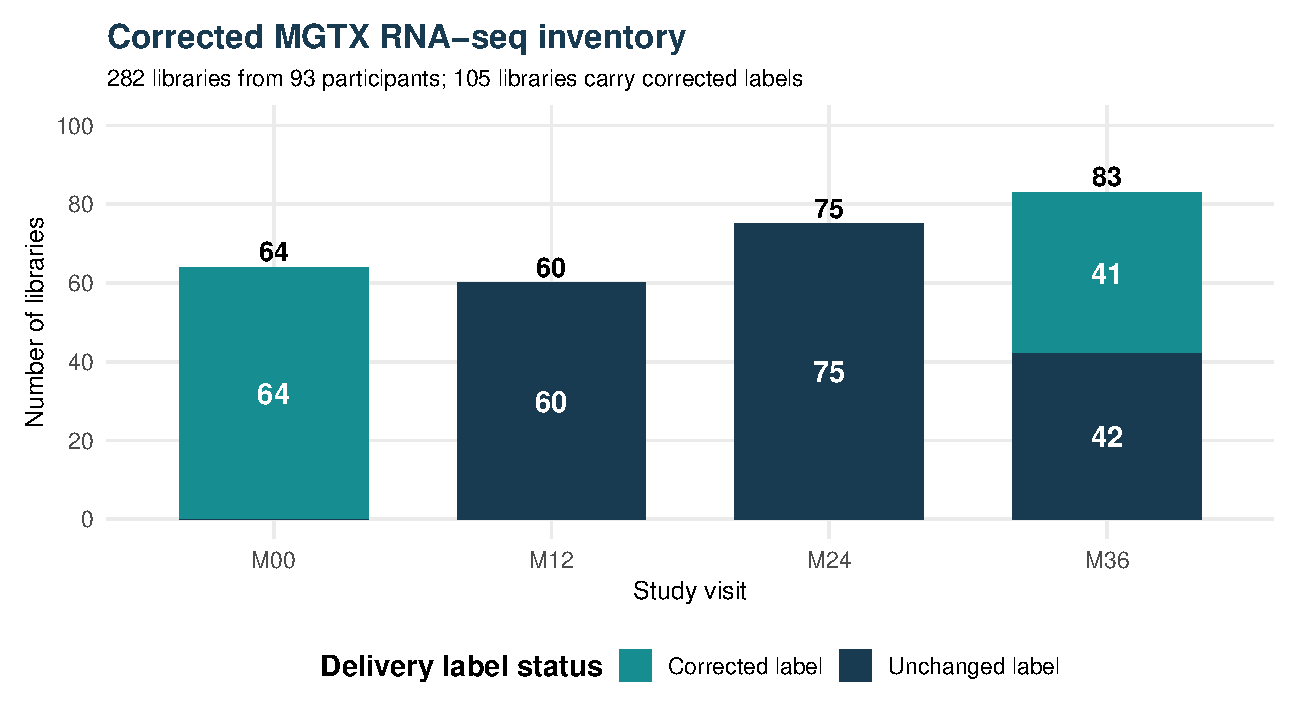
\includegraphics[
			width=\linewidth,
			height=0.70\textheight,
			keepaspectratio
			]{figs/fig01_inventory.pdf}
		\end{center}
		
	\end{columns}
	
	\vspace{0.05cm}
	
	{\scriptsize
		The core's genotype-based reconciliation is documented;
		independent identity verification within the new pipeline
		is still pending.
	}
	
\end{frame}


% ============================================================
% SLIDE 3 -- PROCESSING AND QC COMPLETENESS
% ============================================================

\begin{frame}{Completed preprocessing and quality-control stages}
	
	\vspace{0.2cm}
	
	\begin{columns}[T]
		
		\column{0.48\textwidth}
		
		\begin{block}{Data and integrity checks}
			
			\begin{itemize}
				\item 282 paired-end RNA-seq libraries
				\item 564 FASTQ files transferred
				\item 564/564 passed gzip-integrity validation
				\item 282/282 R1/R2 sequence-count pairs concordant
				\item Four restored V1 R1 files retained with
				checksum-verification history
			\end{itemize}
			
		\end{block}
		
		\column{0.48\textwidth}
		
		\begin{block}{Quality-control analyses}
			
			\begin{itemize}
				\item FastQC completed on all 564 FASTQs
				\item MultiQC integrated all 564 reports
				\item Eleven FastQC modules summarized
				\item Per-tile data examined for all 564 files
				\item Representative original FastQC reports reviewed
			\end{itemize}
			
		\end{block}
		
	\end{columns}
	
	\vspace{0.2cm}
	
	\begin{center}
		\Large
		\textcolor{mgtxteal}{
			\textbf{All 282 libraries passed the initial file-integrity gate}
		}
	\end{center}
	
	\vspace{0.1cm}
	
	\begin{center}
		\small
		Median sequencing depth:
		\textbf{85.3 million read pairs per library}
	\end{center}
	
	\vspace{0.1cm}
	
	{\scriptsize
		These are FASTQ-level technical results.
		They do not establish mapping quality, mate synchronization,
		or participant identity.
	}
	
\end{frame}


% ============================================================
% SLIDE 4 -- FASTQC MODULE STATUS
% ============================================================

\begin{frame}{FastQC: strong base quality, frequent diagnostic flags}
	
	\begin{center}
		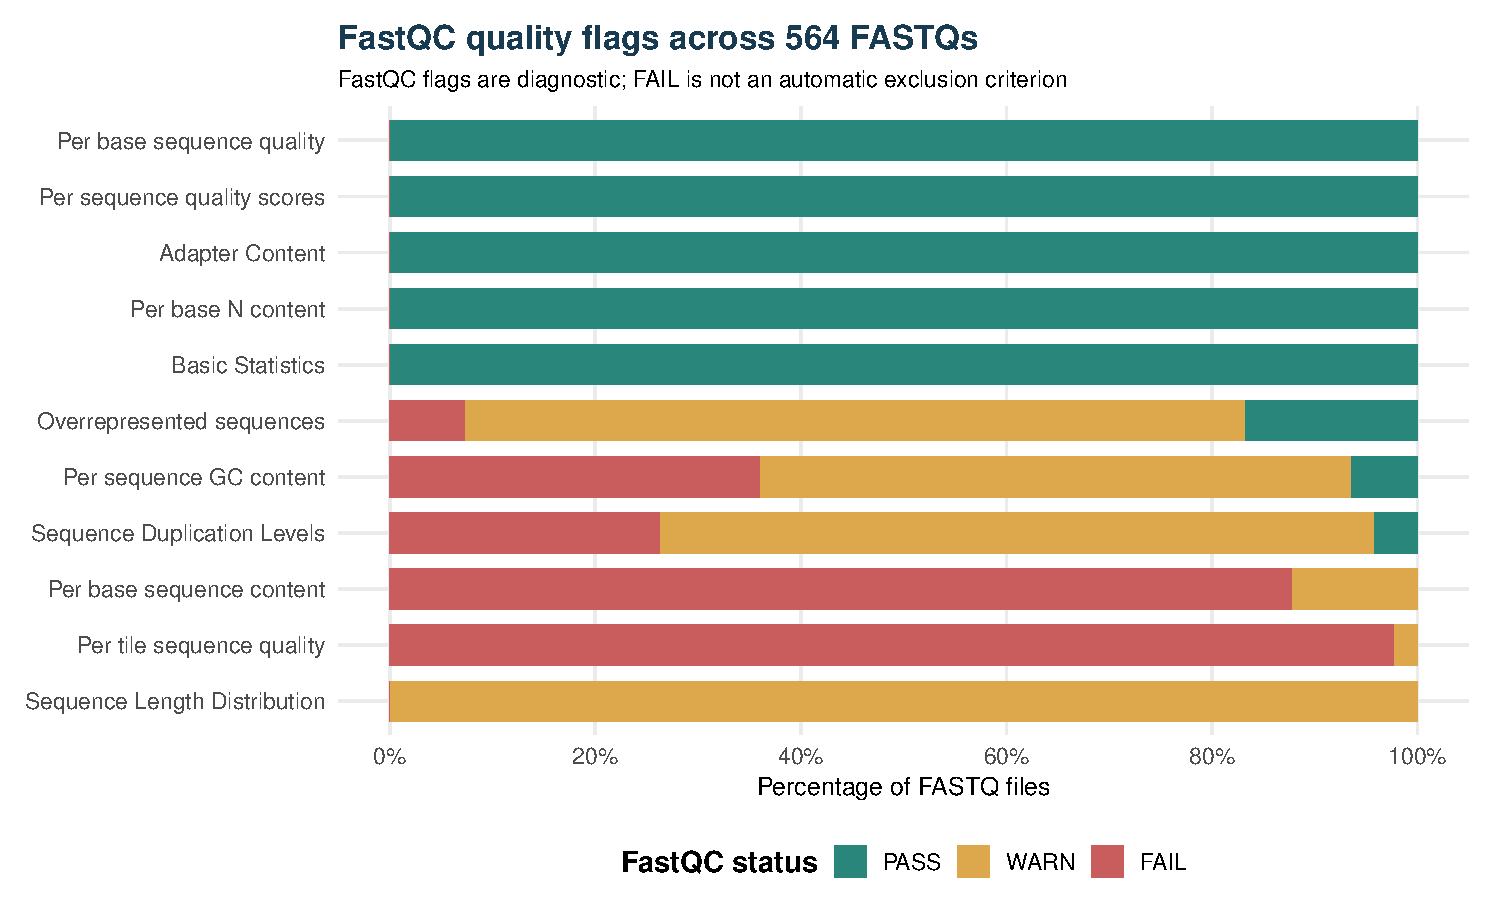
\includegraphics[
		width=0.99\linewidth,
		height=0.7\textheight,
		keepaspectratio
		]{figs/fig02_fastqc_modules.pdf}
	\end{center}
	
	\vspace{-0.4cm}
	
	\small
	\textbf{Key interpretation:}
	All 564 FASTQs passed per-base quality,
	per-sequence quality, adapter-content, and N-content checks.
	
	\smallskip
	
	\textbf{Caution:}
	Per-tile, nucleotide-composition, GC-content,
	and duplication flags require contextual interpretation.
	A FastQC FAIL does not imply that a library is unusable.
	
\end{frame}


% ============================================================
% SLIDE 5 -- TILE-QUALITY INVESTIGATION
% ============================================================

\begin{frame}{High per-tile FAIL rates do not imply widespread damage}
	
	\begin{center}
		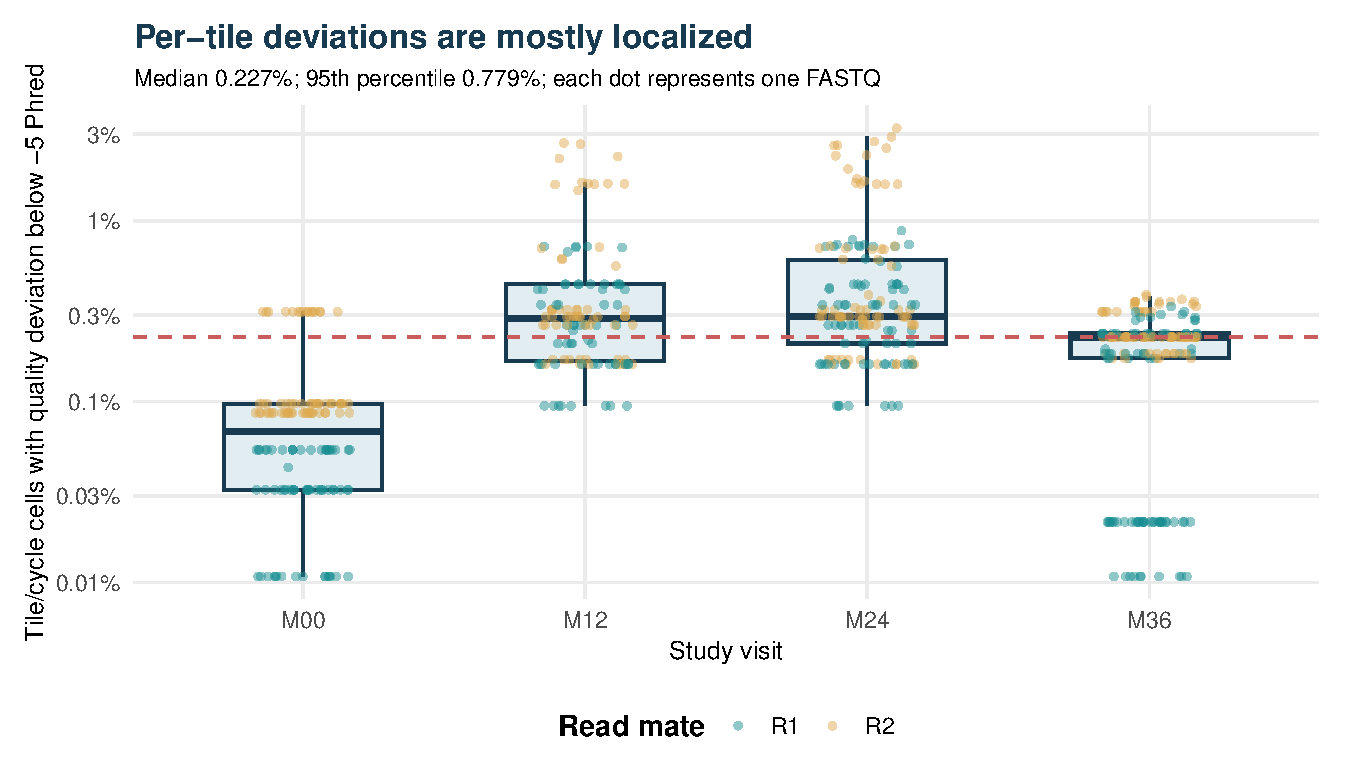
\includegraphics[
		width=0.93\linewidth,
		height=0.60\textheight,
		keepaspectratio
		]{figs/fig03_tile_burden.pdf}
	\end{center}
	
	\vspace{-0.3cm}
	
	\begin{itemize}
		\item \textbf{551/564} FASTQs received per-tile FAIL flags.
		\item Median fraction of tile/cycle cells below
		$-5$ Phred: \textbf{0.227\%}.
		\item 95th percentile: \textbf{0.779\%};
		maximum: \textbf{3.248\%}.
	\end{itemize}
	
	{\scriptsize
		The percentages describe tile/cycle measurements,
		not the percentage of reads affected.
		More pronounced effects occur in selected runs,
		especially the R2 files of Data\_Sequencing 4.
	}
	
\end{frame}


% ============================================================
% SLIDE 6 -- GC CONTENT
% ============================================================

\begin{frame}{GC heterogeneity warrants batch-aware interpretation}
	
	\begin{center}
		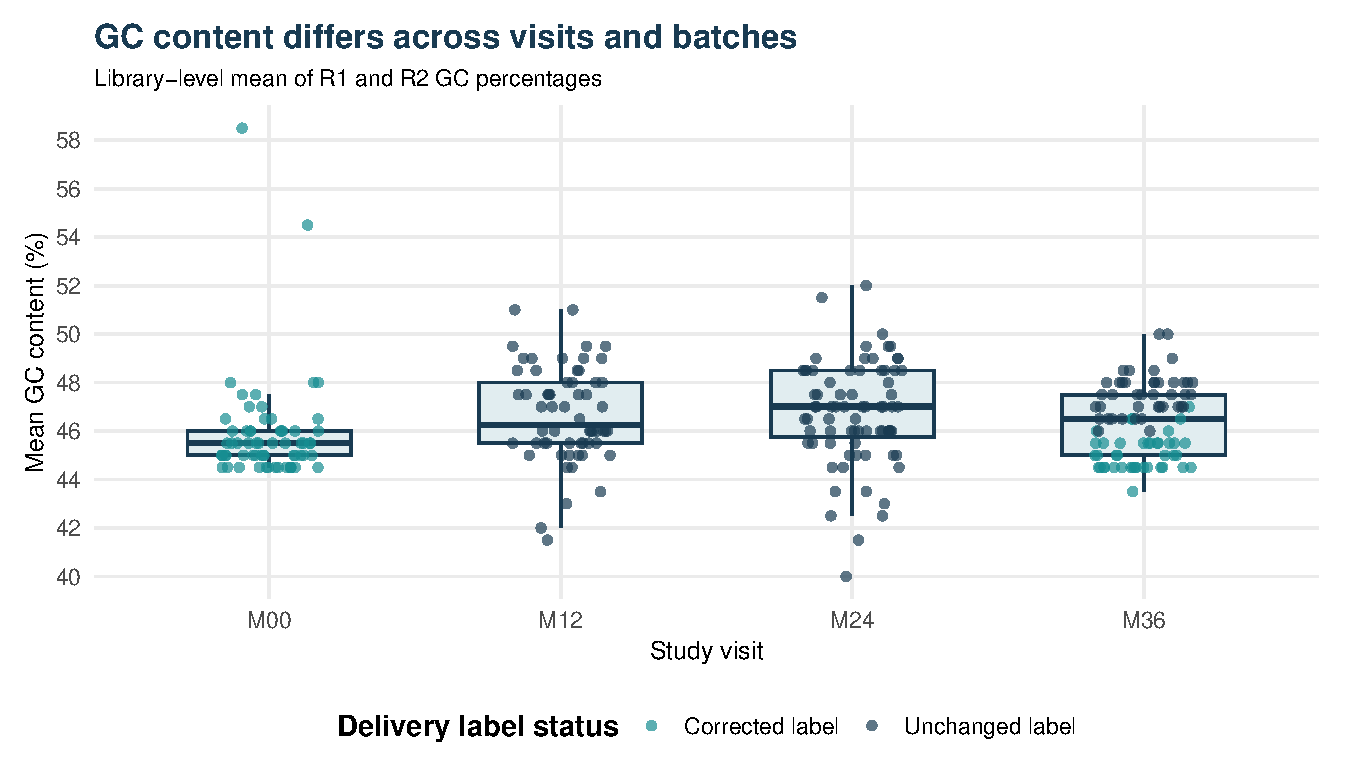
\includegraphics[
		width=0.91\linewidth,
		height=0.69\textheight,
		keepaspectratio
		]{figs/fig04_gc_visits.pdf}
	\end{center}
	
	\vspace{-0.10cm}
	
	\small
	
	\begin{itemize}
		\item Overall median FASTQ GC content was
		approximately \textbf{46\%}.
		
		\item MultiQC showed heterogeneous GC distributions,
		including secondary peaks in some libraries.
		
		\item Corrected-label and unchanged-label libraries
		differ in visit and sequencing-run composition.
	\end{itemize}
	
	\textbf{Interpretation:}
	Observed GC differences cannot be attributed to
	sample relabeling itself. STAR alignment and
	overrepresented-sequence assessment are needed.
	
\end{frame}


% ============================================================
% SLIDE 7 -- READ LENGTH AND TECHNICAL SIGNATURES
% ============================================================

\begin{frame}{Read-length differences indicate batch-specific signatures}
	
	\begin{center}
		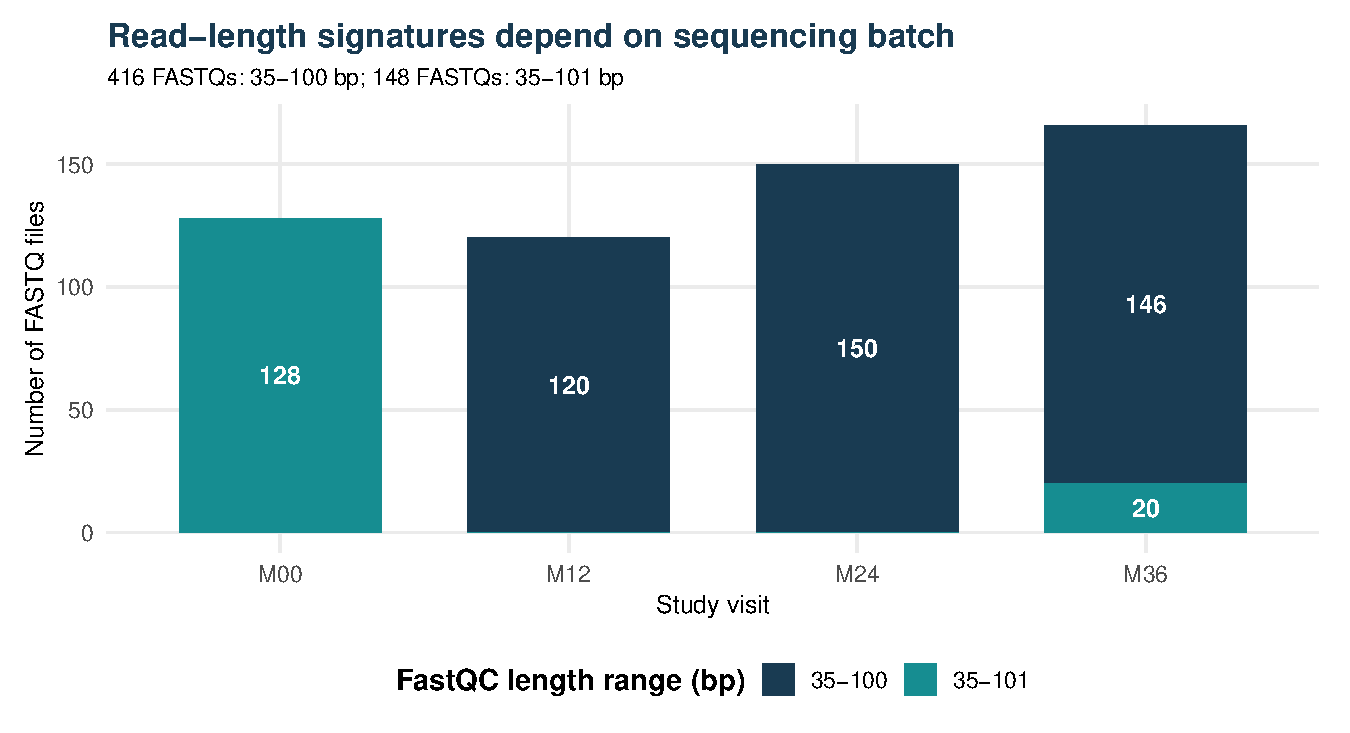
\includegraphics[
		width=0.92\linewidth,
		height=0.67\textheight,
		keepaspectratio
		]{figs/fig05_read_lengths.pdf}
	\end{center}
	
	\vspace{-0.05cm}
	
	\small
	
	\begin{itemize}
		\item 416 FASTQs had a reported length range of
		35--100 bp; 148 had 35--101 bp.
		
		\item In the 35--100 bp group, FastQC reported
		0\% cytosine at the terminal position.
		
		\item The source and significance of this signature
		require review of preprocessing records.
	\end{itemize}
	
	{\scriptsize
		These are per-file FastQC length ranges, not the
		distribution of individual read lengths.
		No library is excluded on this basis.
	}
	
\end{frame}


% ============================================================
% SLIDE 8 -- KEEP VS EXCLUDE DECISION
% ============================================================

\begin{frame}{Should we exclude libraries before STAR?}
	
	\begin{columns}[T]
		
		\column{0.49\textwidth}
		
		\begin{block}{Option A: Retain all 282 for mapping}
			
			\small
			
			\textbf{\textcolor{mgtxteal}{Recommended}}
			
			\medskip
			
			\textbf{Benefits}
			\begin{itemize}
				\item Preserves available longitudinal samples
				\item Avoids selection driven by generic FastQC flags
				\item Reduces risk of batch-dependent exclusions
				\item Allows alignment metrics to inform exclusions
			\end{itemize}
			
			\textbf{Costs}
			\begin{itemize}
				\item Additional HPC time and storage
				\item More downstream QC and identity checks
				\item Some libraries may ultimately be excluded
			\end{itemize}
			
		\end{block}
		
		\column{0.49\textwidth}
		
		\begin{block}{Option B: Exclude on FastQC FAIL}
			
			\small
			
			\textbf{\textcolor{mgtxred}{Not recommended}}
			
			\medskip
			
			\textbf{Potential benefit}
			\begin{itemize}
				\item Reduces processing of known poor-quality
				libraries when defects are substantial
			\end{itemize}
			
			\textbf{Problems in this dataset}
			\begin{itemize}
				\item Every library has at least one FastQC FAIL
				\item A blanket rule would discard all 282 libraries
				\item Many flags are common or localized
				\item Exclusions may disproportionately affect
				specific runs and study visits
			\end{itemize}
			
		\end{block}
		
	\end{columns}
	
	\vspace{0.16cm}
	
	\begin{center}
		\textbf{
			Decision: Map all 282 libraries first;
			decide analysis eligibility after alignment and identity QC.
		}
	\end{center}
	
\end{frame}


% ============================================================
% SLIDE 9 -- REANALYSIS ROADMAP / PI DECISION
% ============================================================

\begin{frame}{Next steps and decisions for the MGTX analysis}
	
	\begin{enumerate}
		
		\item \textbf{STAR alignment of all 282 libraries}
		
		\begin{itemize}
			\item Two-library pilot submitted for resource
			and mapping validation
			\item Planned resources: 8 CPUs, 56 GB RAM per job
			\item Maximum 20 concurrent array tasks
		\end{itemize}
		
		\vspace{0.13cm}
		
		\item \textbf{Alignment-based QC}
		
		\begin{itemize}
			\item Uniquely mapped reads and multimapping
			\item Gene assignment and strand orientation
			\item Batch-specific mapping differences
			\item Unusual sequences and possible contamination
		\end{itemize}
		
		\vspace{0.13cm}
		
		\item \textbf{Independent longitudinal sample-identity QC}
		
		\begin{itemize}
			\item SNP fingerprints across repeated visits
			\item Concordance with the documented corrected labels
			\item Preserve an auditable mapping of identifiers
		\end{itemize}
		
		\vspace{0.13cm}
		
		\item \textbf{Clinical linkage and differential expression}
		
		\begin{itemize}
			\item Define the eligible longitudinal analysis subset
			\item Rerun cpGLMM and relevant sensitivity analyses
			\item Compare corrected results with previous findings
		\end{itemize}
		
	\end{enumerate}
	
	\begin{block}{Proposed decision for PI discussion}
		Proceed with all 282 technical libraries for initial alignment.
		Defer exclusion and final manuscript updates until
		alignment QC and independent identity verification are complete.
	\end{block}
	
\end{frame}








\begin{frame}{Today in one slide}
  \begin{itemize}
    \item \textbf{Question:} which genes change their activity across a tissue section, beyond simply
          reflecting which tissue type is where?
    \item \textbf{Tool:} a new statistical method (Mingcong Wu. Yang Li. Shuangge Ma. Mengyun Wu. "Joint identification of spatially variable genes via a network-assisted Bayesian regularization approach." Ann. Appl. Stat. 19 (4) 2705 - 2723, December 2025.).
    \item \textbf{What I did:} built simulated tissue with known ground truth, and tested the method.
    \item \textbf{Result:} it ranks genes very well, but its yes/no calls produce too many false alarms
          on data as sparse as ours. \textcolor{red}{We know where the false alarms come from.}
  \end{itemize}
\end{frame}

% =====================================================================
\section{Background}

\begin{frame}{Spatial transcriptomics in one picture}
  \begin{itemize}
    \item A tissue section is divided into tiny squares (``bins'', 16\,$\mu$m, roughly cell-sized).
    \item For each bin we count the RNA molecules of $\sim$18{,}000 genes.
    \item For each bin we also know its \textbf{tissue type}: epithelium, stroma, fat, immune cells, vessels.
    \item A \textbf{spatially variable gene} is one whose activity forms a pattern across the tissue:
          a gradient, a hotspot, a band.
  \end{itemize}
\end{frame}

\begin{frame}{The trap: tissue layout looks like a spatial pattern}
  \begin{itemize}
    \item Fat sits in one region of the section, epithelium in others.
    \item A gene that is active only in fat will therefore \emph{look} spatial but it simply marks fat.
    \item We want genes whose pattern goes \textbf{beyond} the tissue layout
          (e.g.\ a gradient \emph{within} stroma).
    \item The method we tested is designed to correct for tissue type, and it also uses known
          gene--gene interactions: genes that work together are assessed together.
  \end{itemize}
\end{frame}

\begin{frame}{Why test on simulated tissue first?}
  \begin{itemize}
    \item On real samples we do not know which genes are truly spatial.
    \item In simulated tissue we \textbf{decide the truth}, so we can grade the method (like validating a diagnostic test on samples with a known diagnosis).
  \end{itemize}
  \vspace{3mm}
  \centering
  \begin{tabular}{ll}
    \toprule
    Statistical term & Clinical equivalent \\
    \midrule
    Recall & Sensitivity: true spatial genes that are found \\
    Precision & Positive predictive value (PPV): flagged genes that are truly spatial \\
    AUROC & Area under the ROC curve: quality of the ranking ({\small 0.5 = coin flip, 1 = perfect}) \\
    \bottomrule
  \end{tabular}
\end{frame}

% =====================================================================
\section{Simulated tissue}

\begin{frame}{Our simulated tissue, modelled on our data}
  \begin{columns}[T]
    \begin{column}{0.58\textwidth}
      \safegraphic{width=\linewidth,height=0.75\textheight,keepaspectratio}{figs/tissue.png}
    \end{column}
    \begin{column}{0.40\textwidth}
      \small
      \begin{itemize}
        \item \res{fig-nbins} bins, \res{fig-ngenes} genes.
        \item Six tissue types, arranged like a real section.
        \item Fat lobe on one side, epithelial islands, immune clusters, thin vessels.
      \end{itemize}
    \end{column}
  \end{columns}
\end{frame}

\begin{frame}{Fat carries much less RNA}
	\begin{columns}[T]
		\begin{column}{.7\textwidth}
			\centering
			\safegraphic{height=.8\textheight,keepaspectratio}{figs/qc.png}
		\end{column}
		\begin{column}{.3\textwidth}
			\vspace{2cm}Fat bins have far fewer RNA molecules and detected genes; as in real adipose tissue.
		\end{column}
	\end{columns}
\end{frame}

\begin{frame}{The answer key we built in}
  \centering
  \safegraphic{width=\linewidth,height=0.62\textheight,keepaspectratio}{figs/truth.png}
  \small
  \begin{itemize}
    \item \textbf{True spatial genes}: gradients, waves, hotspots (top row).
    \item \textbf{Decoys}: tissue-type markers that only \emph{look} spatial. These should \emph{not} be flagged and we treat them as \textcolor{red}{false positive}.
  \end{itemize}
\end{frame}

% =====================================================================
\section{Results}

\begin{frame}{Result 1: too many false alarms on data like ours}
  \begin{itemize}
    \item As published: sensitivity \res{A-rec}, PPV \res{A-prec}.
    \item Best version we tried: sensitivity \res{E-rec}, PPV \res{E-prec}.
    \item In plain words: most genes the method flags are \textbf{not} truly spatial.
  \end{itemize}
  \vspace{3mm}
  \small Fits used a smaller version of the simulated tissue (\res{fit-nbins} bins, \res{fit-ngenes} genes),
  with neighbouring bins combined into larger squares to boost the signal.
\end{frame}

\begin{frame}{Result 2: the tissue-type correction works}
  \centering
  \safegraphic{width=\linewidth,height=0.6\textheight,keepaspectratio}{figs/callrate.pdf}
  \small
  \begin{itemize}
    \item Decoy markers are flagged no more often than ordinary non-spatial genes
          (\res{B-rate-marker} vs.\ \res{B-rate-null}).
    \item So the false alarms are \emph{not} caused by the tissue layout. Bars are different versions of the method.
  \end{itemize}
\end{frame}

\begin{frame}{Result 3: the ranking is useful}
  \centering
  \safegraphic{width=\linewidth,height=0.62\textheight,keepaspectratio}{figs/topk.pdf}
  \small
  \begin{itemize}
    \item Left: our data. The genes ranked at the very top are almost all truly spatial;
          accuracy falls further down the list (overall AUROC \res{D-aucb-ALL}).
    \item Right: the authors' simulation design, where the ranking is close to perfect.
  \end{itemize}
\end{frame}

\begin{frame}{Result 4: on the authors' own simulation design}
  \begin{itemize}
    \item We rebuilt the simulation described in the paper and ran our implementation on it.
    \item \textbf{All} \res{F-ntrue} truly spatial genes found (sensitivity \res{F-rec}).
    \item Ranking almost perfect: AUROC \res{F-aucbeta}.
    \item PPV \res{F-prec}; the authors report \res{paper-prec} with longer, repeated runs that we could
          not do on a laptop.
  \end{itemize}
  \vspace{3mm}
  $\Rightarrow$ The method works as described. The problems appear on data like ours.
\end{frame}

\begin{frame}{Why the difference? Two reasons}
  \begin{enumerate}
    \item \textbf{Our data are much sparser.} Median reads per gene per location:
          \res{paper-cpg} in the authors' design vs.\ \res{ours-cpg} in ours ---
          like running a test on a much smaller sample.
    \item \textbf{One specific weak spot.} Most remaining false alarms on the authors' design
          (\res{F-nullhub} of \res{F-fp}) are ``hub'' genes --- genes with many connections in the
          gene network. This points to one step of the method that we can fix.
  \end{enumerate}
\end{frame}

% =====================================================================
\section{Conclusions}

\begin{frame}{Take-home messages}
  \begin{enumerate}
    \item The method correctly accounts for tissue type --- the main pitfall for our question.
    \item It ranks genes well, especially on data with enough signal.
    \item Its automatic yes/no calls are not yet reliable on data as sparse as ours.
    \item We have identified concrete causes (sparsity, hub genes) and how to address them.
  \end{enumerate}
\end{frame}

\begin{frame}{What this means for our samples}
  \begin{itemize}
    \item \textbf{Combine neighbouring bins} into larger squares to increase the signal.
    \item \textbf{Use the ranking}, not the automatic yes/no calls; follow up the top genes.
    \item \textbf{Add a calibration step} that estimates how many flagged genes are false alarms.
    \item \textbf{Compare} with established tools on the same simulated tissue before analysing patient samples.
  \end{itemize}
\end{frame}

\begin{frame}
  \centering \Large Thank you --- questions?
\end{frame}

% =====================================================================
\appendix

\begin{frame}{Backup: the statistical model}
  \begin{align*}
    Y_{ij} &\sim (1-r_{ij})\,\mathrm{NB}(c_i\mu_{ij},\,\phi) + r_{ij}\,\delta_0,
           \qquad r_{ij}\sim\mathrm{Bern}(\pi_j)\\[2mm]
    \log\mu_{ij} &= \mu_{0j} + \beta^{(1)}_j\,\mathcal K(x_{i1}) + \beta^{(2)}_j\,\mathcal K(x_{i2})
           + \textstyle\sum_{k=1}^{K}\alpha_k\,w_{ik}
  \end{align*}
  \begin{itemize}
    \item $w_{ik}$: tissue-type composition; $\mathcal K$: linear, exponential or periodic kernel.
    \item Gene $j$ is spatially variable $\iff \beta^{(1)}_j\neq0$ or $\beta^{(2)}_j\neq0$.
  \end{itemize}
\end{frame}

\begin{frame}{Backup: prior and inference}
  \begin{align*}
    \boldsymbol\beta &= \boldsymbol\gamma\circ\mathbf 1\{|\boldsymbol\gamma|>\lambda\boldsymbol\rho\},
    &\boldsymbol\gamma &\sim N\big(\mathbf 0,\ \sigma^2_\gamma(\mathbf L+\varepsilon\mathbf I)^{-1}\big),
    &\rho_j &= \Big(\max_{l\in V_{s(j)}}|\gamma_l|\Big)^{-1/2}
  \end{align*}
  \small
  \begin{itemize}
    \item $\mathbf L$: signed, normalized graph Laplacian of the gene network.
    \item MCMC (Gibbs, Metropolis--Hastings, pCN-Langevin); 5 kernels combined; Bayesian FDR 0.05;
          5 chains, genes kept if selected in $\geq80\%$.
    \item Our implementation: Python/PyTorch, about 1\,s per iteration for 1{,}024 spots $\times$ 5{,}000 genes on a laptop CPU.
  \end{itemize}
\end{frame}

\begin{frame}{Backup: all runs on our simulated data}
  \centering
  \resizebox{\linewidth}{!}{\safeinput{tables/runs_ours.tex}}
  \vspace{2mm}
  \small $\rho$: the method's group-wise weighting step. AUC$_{|\hat\beta|}$: ranking by estimated effect size.
\end{frame}

\begin{frame}{Backup: ranking quality by pattern type}
  \centering
  \safegraphic{width=\linewidth,height=0.75\textheight,keepaspectratio}{figs/auc_pattern.pdf}
\end{frame}

\begin{frame}{Backup: replication of the authors' design}
  \centering
  \resizebox{\linewidth}{!}{\safeinput{tables/runs_paper.tex}}
  \vspace{2mm}
  \safegraphic{width=0.9\linewidth,height=0.4\textheight,keepaspectratio}{figs/paper_design.pdf}
\end{frame}

\begin{frame}{Backup: where the false alarms come from}
  \centering
  \safegraphic{width=0.85\linewidth,height=0.55\textheight,keepaspectratio}{figs/hub_ablation.pdf}
  \small
  \begin{itemize}
    \item With the weighting step $\rho$: \res{F-nullhub}/\res{F-nnullhub} non-spatial hub genes and
          \res{F-nonhub}/\res{F-nnonhub} other non-spatial genes flagged.
    \item Without it: \res{G-nullhub}/\res{G-nnullhub} and \res{G-nonhub}/\res{G-nnonhub}.
          $\rho$ silences noise in ordinary genes but promotes hubs.
  \end{itemize}
\end{frame}

\begin{frame}{Backup: candidate mechanism (hypothesis)}
  \begin{columns}[T]
    \begin{column}{0.55\textwidth}
      \safegraphic{width=\linewidth,height=0.7\textheight,keepaspectratio}{figs/mechanism.pdf}
    \end{column}
    \begin{column}{0.43\textwidth}
      \small
      If hub $h$ has the largest $|\gamma|$ in its sub-network, $\rho_h=|\gamma_h|^{-1/2}$, so
      $h$ is selected $\iff |\gamma_h|>\lambda^{2/3}$.
      Observed: $\lambda^{2/3}=\res{F-lam23}$; flagged non-spatial hubs have median
      $|\hat\beta|=\res{F-fphub}$.
    \end{column}
  \end{columns}
\end{frame}

\begin{frame}{Backup: gene network view (authors' design)}
  \centering
  \safegraphic{width=\linewidth,height=0.8\textheight,keepaspectratio}{figs/network_paper.png}
\end{frame}

\begin{frame}{Backup: MCMC traces}
  \centering
  \safegraphic{width=\linewidth,height=0.6\textheight,keepaspectratio}{figs/traces_paper.pdf}
\end{frame}

\end{document}
